\documentclass[12pt]{beamer}
\usetheme{Rochester}
\usepackage[utf8]{inputenc}
\usepackage{amsmath}
\usepackage{amsfonts}
\usepackage{amssymb}
\usepackage{graphicx}
\usepackage{makecmds}
\usepackage{movie15}


\DeclareGraphicsExtensions{.pdf,.png,.jpg}

\author{Kyle Treleaven}
\title{State-space, Equilibria, and Stability and Lyapunov Methods I}
%\setbeamercovered{transparent} 
%\setbeamertemplate{navigation symbols}{} 
%\logo{} 
%\institute{} 
\date{Friday, Jan.~9, 2015} 
\subject{Lunch \& Learn} 

\usefonttheme[onlymath]{serif}

% typesetting
\makecommand{\vitem}{\vfill\item}

% general math
\makecommand{\reals}{{\mathbb R}}
\makecommand{\timederiv}{\frac{d}{dt}}
\makecommand{\onehalf}{\frac{1}{2}}
\makecommand{\xpose}{{\rm T}}
\makecommand{\vecnorm}[1]{\left\|#1\right\|}

% specific math
\makecommand{\zerovec}{{\bf 0}}

\makecommand{\vecu}{{\bf u}}
\makecommand{\vecx}{{\bf x}}
\makecommand{\matA}{{\bf A}}
\makecommand{\matC}{{\bf C}}
\makecommand{\vectheta}{{\boldsymbol\theta}}

\begin{document}

\begin{frame}
\titlepage

\end{frame}

%\begin{frame}
%\tableofcontents
%\end{frame}




\section{State-space}


\begin{frame}
\vfill
\centering
{\Large State Space: Redux}
\vfill\null
\end{frame}


\begin{frame}
%\frametitle{State-space Philosophy}
\centering
\vfill
%\includegraphics[width=.6\linewidth]{pic/tennis-ball-650x487.jpeg}
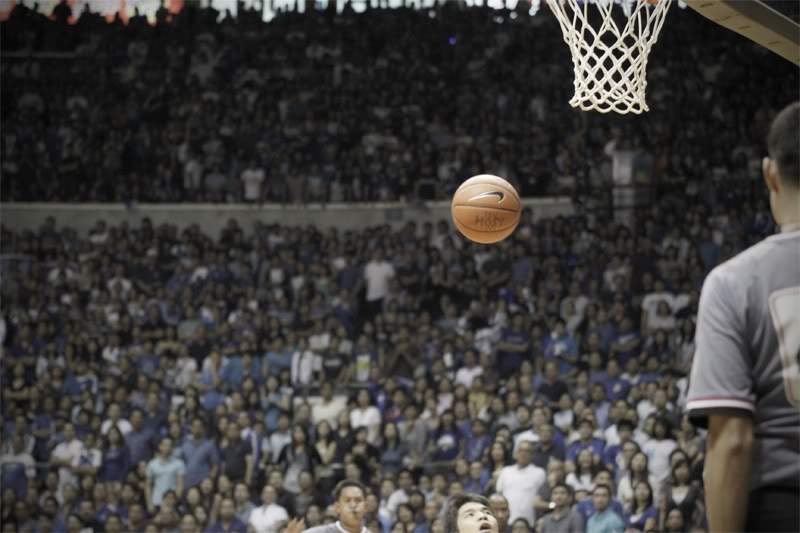
\includegraphics[width=.6\linewidth]{pic/airball.jpg}

Where's the ball going to go?
\vfill\null
\end{frame}





\begin{frame}
\frametitle{State-space Philosophy}

\begin{itemize}

\vitem Clearly, position is not all the information that is needed to determine trajectory.

\vitem But, the ball couldn't do just anything; only certain kinds of trajectories are possible.

\end{itemize}

\vfill\null
\end{frame}





\begin{frame}
\frametitle{State-space Philosophy}
%(1. Draw many possible trajectories of a bouncing ball)

\begin{columns}

\column{.6\linewidth}
\centering
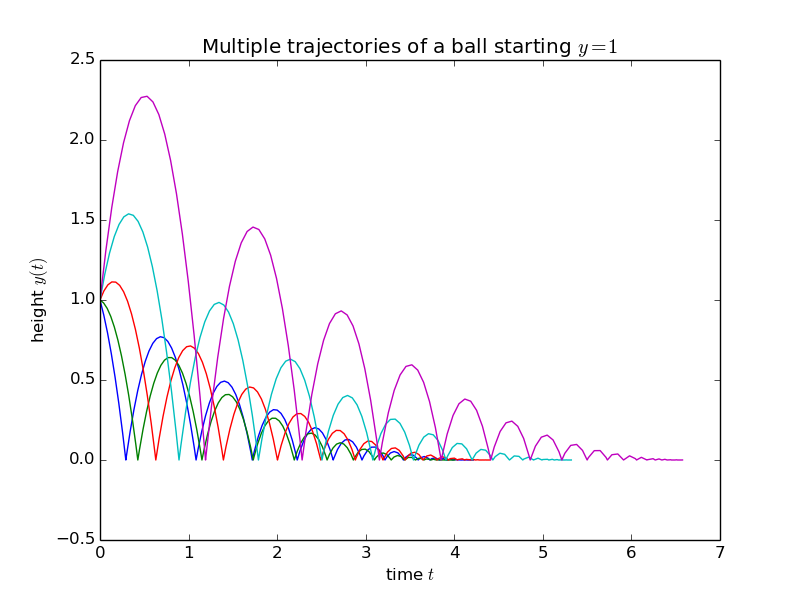
\includegraphics[width=\linewidth]{pic/bouncing_ball_flat}

Infinitely many trajectories of a ball

(under influence of gravity)

\column{.35\linewidth}
\centering
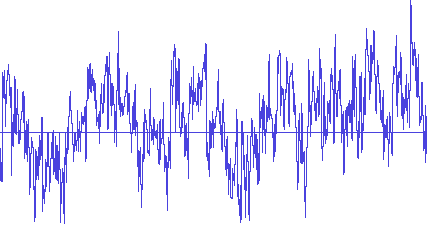
\includegraphics[width=\linewidth]{pic/pink.png}

(But not arbitrary)

\end{columns}

%\begin{block}{Problem}
%may exhibit many trajectories possbile from a particular location, of a bouncing ball under gravity.
%\end{block}

\end{frame}












\begin{frame}
\frametitle{Bouncing Ball Ideal Model}

\begin{block}{Continuous dynamics}
\begin{itemize}
\vitem
$\ddot x = -g$ (free fall)
\end{itemize}
\end{block}

\begin{block}{``Jump'' dynamics}
\begin{itemize}
\vitem
Whenever $x = 0$ and $\dot x < 0$

\vitem
Then, (bounce)
\[
\begin{cases}
x^+ = x	\\
\dot x^+ = -\gamma \dot x
\end{cases}
\]
\end{itemize}
\end{block}

\end{frame}




\begin{frame}
\frametitle{Bouncing Ball Trajectories (Solution)}
\fontsize{10pt}{7.2}\selectfont
\begin{itemize}
\vitem
Trajectory during initial \emph{free-fall} \\
$y(t) = y(0) + \dot y(0) \, t - \onehalf \ g \, t^2$

\vitem
Time of the initial bounce \\
$t_0 = g^{-1} \left( \dot y(0) + \sqrt{ 2g \, y(0) + \dot y^2(0)} \right)$

\vitem
Velocity immediately \emph{after} $k$-th bounce \\
$\dot y(t_k^+) = \gamma^k \sqrt{ 2g \, y(0) + \dot y^2(0) }$

\vitem
Time of each subsequent bounce \\
$t_k = t_0 + (2/g) \ \dot y(t_0^+) \ [1-\gamma^k ]/(1-\gamma)$

\vitem Trajectory during $(k+1)$-th \emph{free-fall} \\
$y(t) = \dot y(t_k^+) \ t' - \onehalf \ g \, t'^2$ \hfill (for $t_k \leq t < t_{k+1}$, $t' = t - t_k$)

\end{itemize}

\end{frame}












\begin{frame}

\centering
\emph{Trajectories determined by $y(0)$ and $\dot y(0)$ \emph{alone}!}

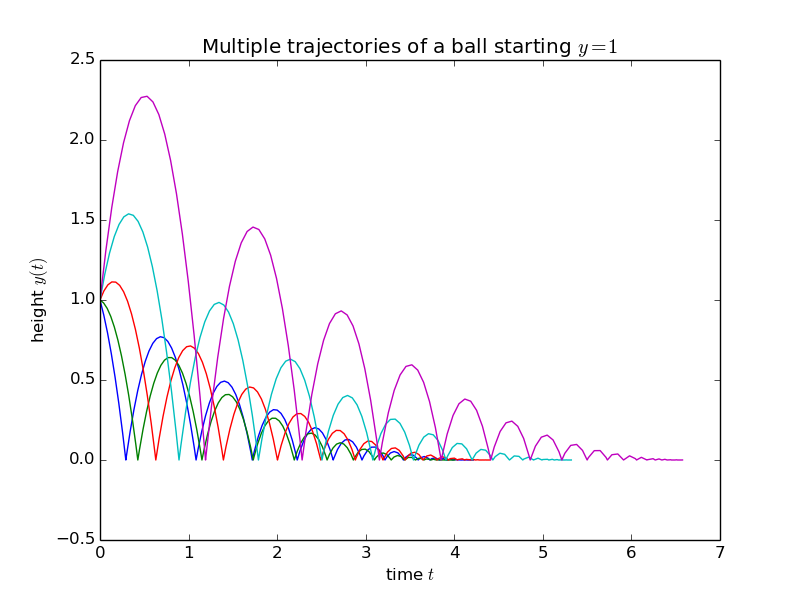
\includegraphics[width=.7\linewidth]{pic/bouncing_ball_flat}

$y(0)=1$, $\dot y(0)$ various

\end{frame}




\begin{frame}
\frametitle{A Bouncing Ball ``State-Space''}
\begin{itemize}
%\vitem Associating a ``velocity'' with the ball gives enough information to determine the future trajectory.

\vitem $(y(t),\dot y(t))$, combination of position and velocity,
\emph{provides enough information to determine the whole future(s)}.

\vitem ...essential unit of information we call \emph{state}.

%\vitem Every possible trajectory can be recovered using some \emph{initial condition} $x_0$.
\end{itemize}

\vfill\null
\end{frame}



\begin{frame}
\vfill\centering
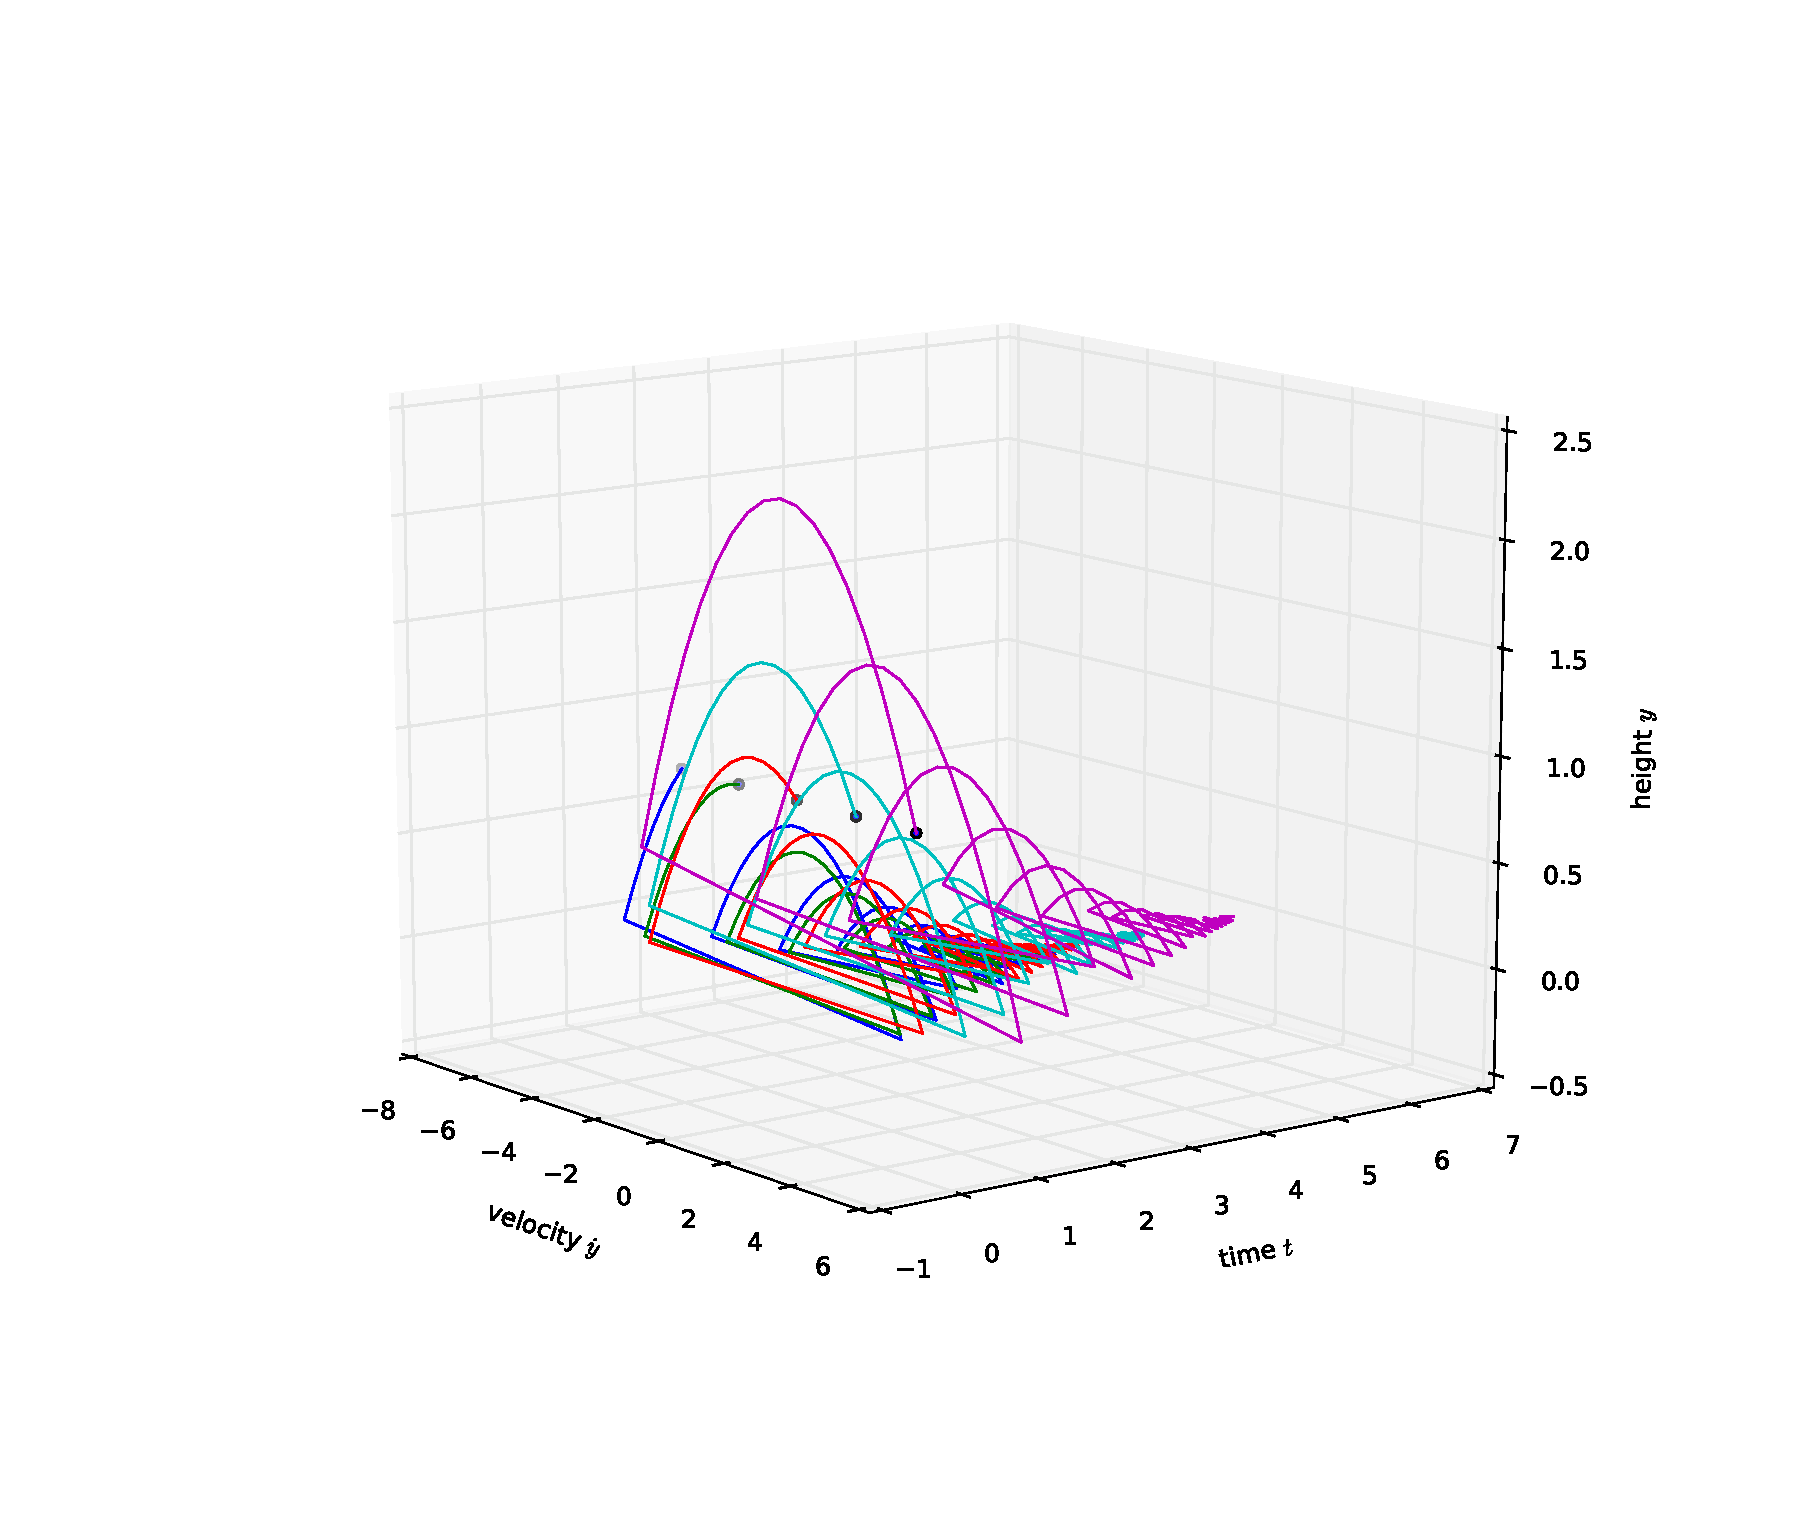
\includegraphics[width=.9\linewidth]{pic/bouncing_ball_deflattened}
\vfill\null
\end{frame}
\begin{frame}
\vfill\centering
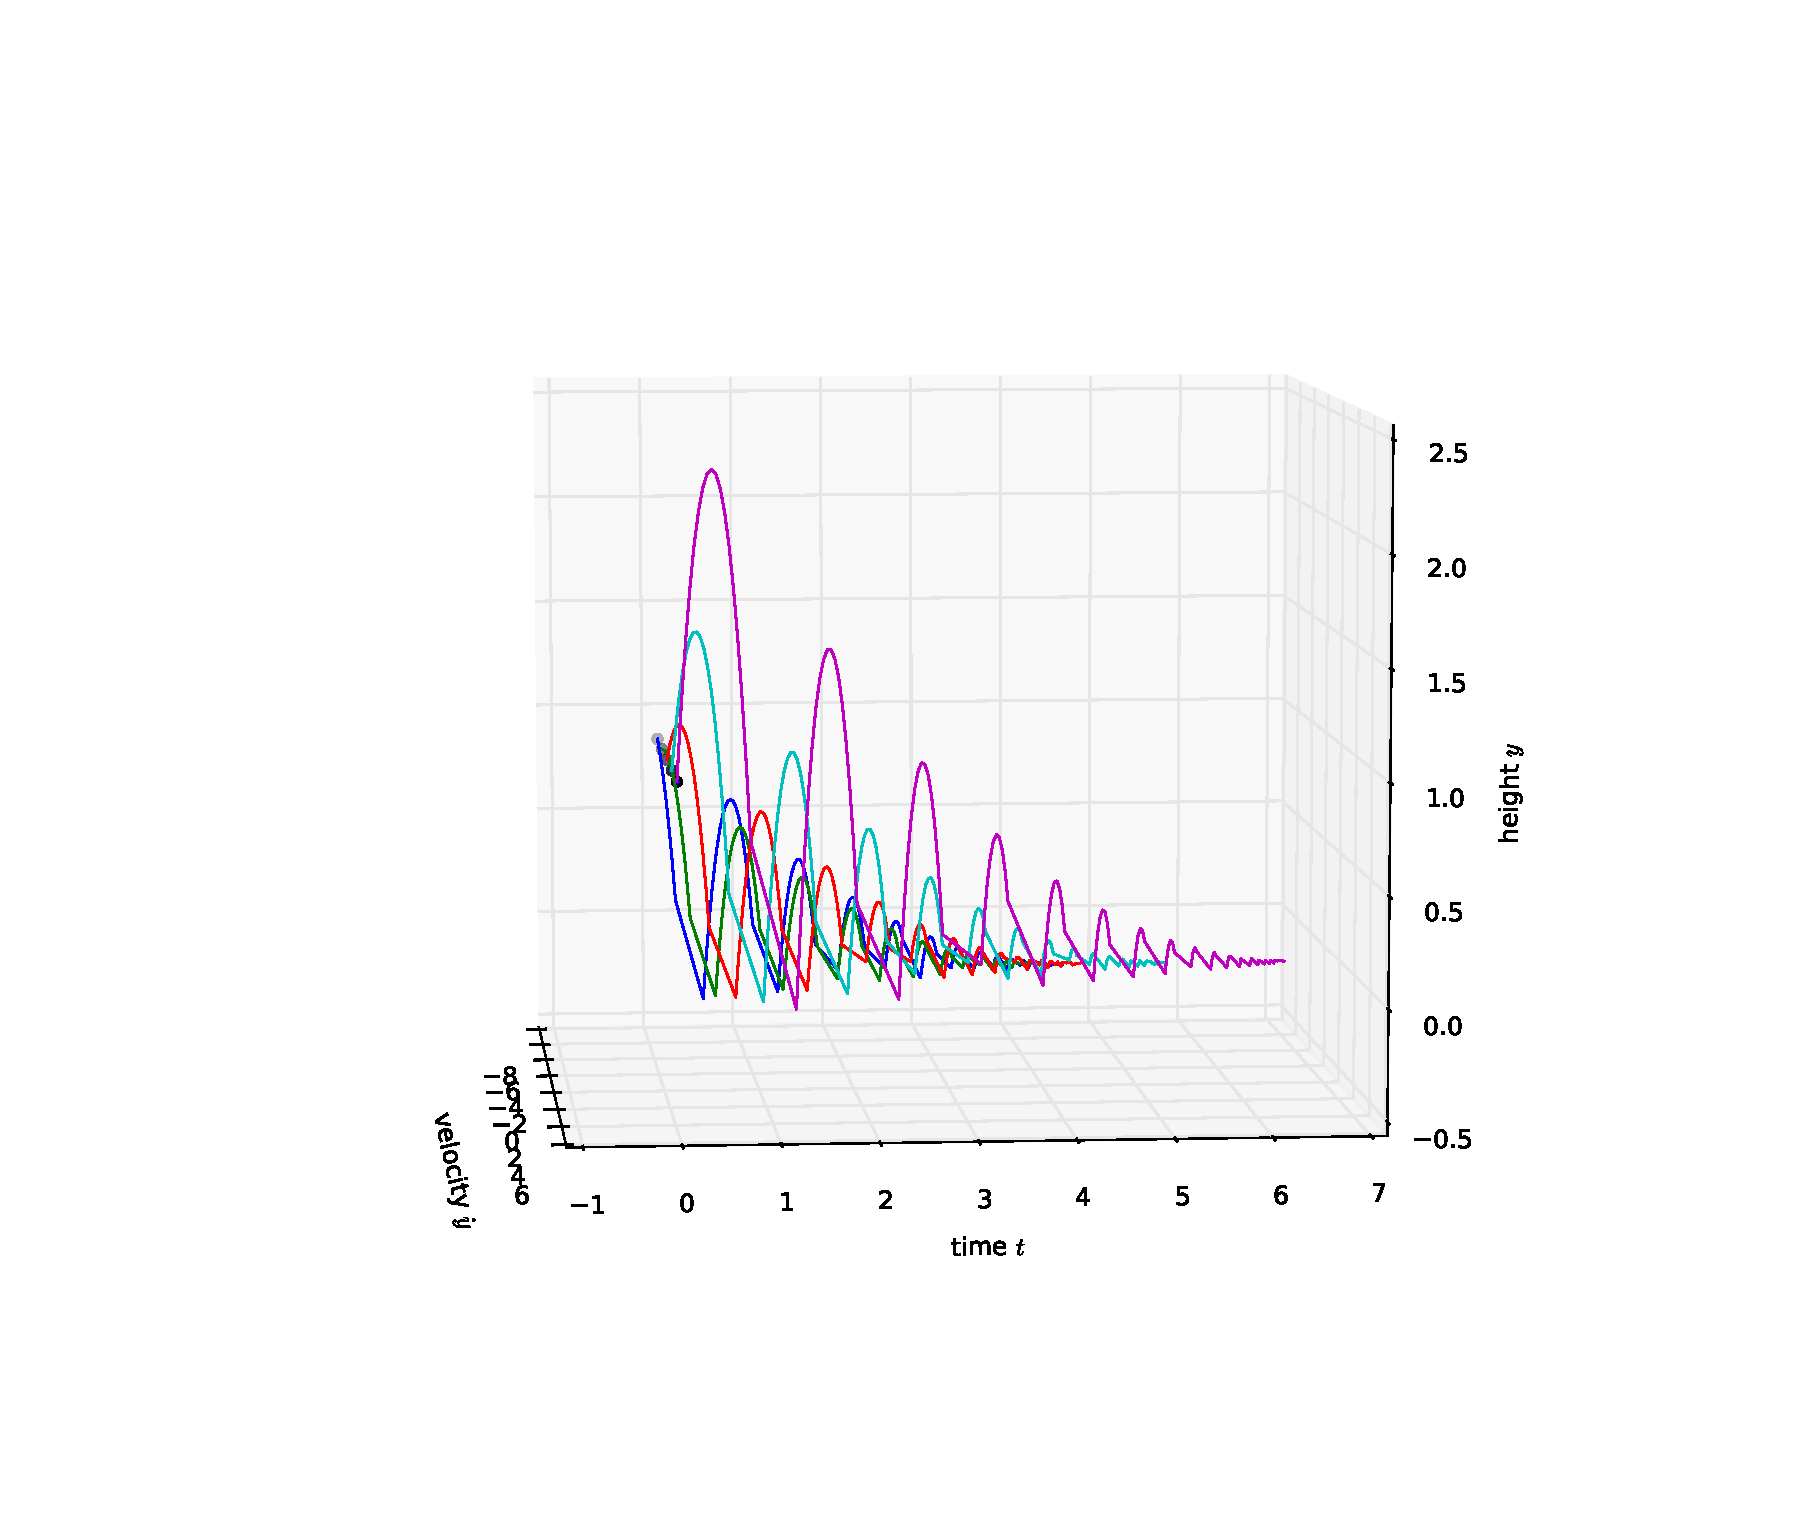
\includegraphics[width=.9\linewidth]{pic/bouncing_ball_deflattened2}
\vfill\null
\end{frame}
\begin{frame}
\vfill\centering
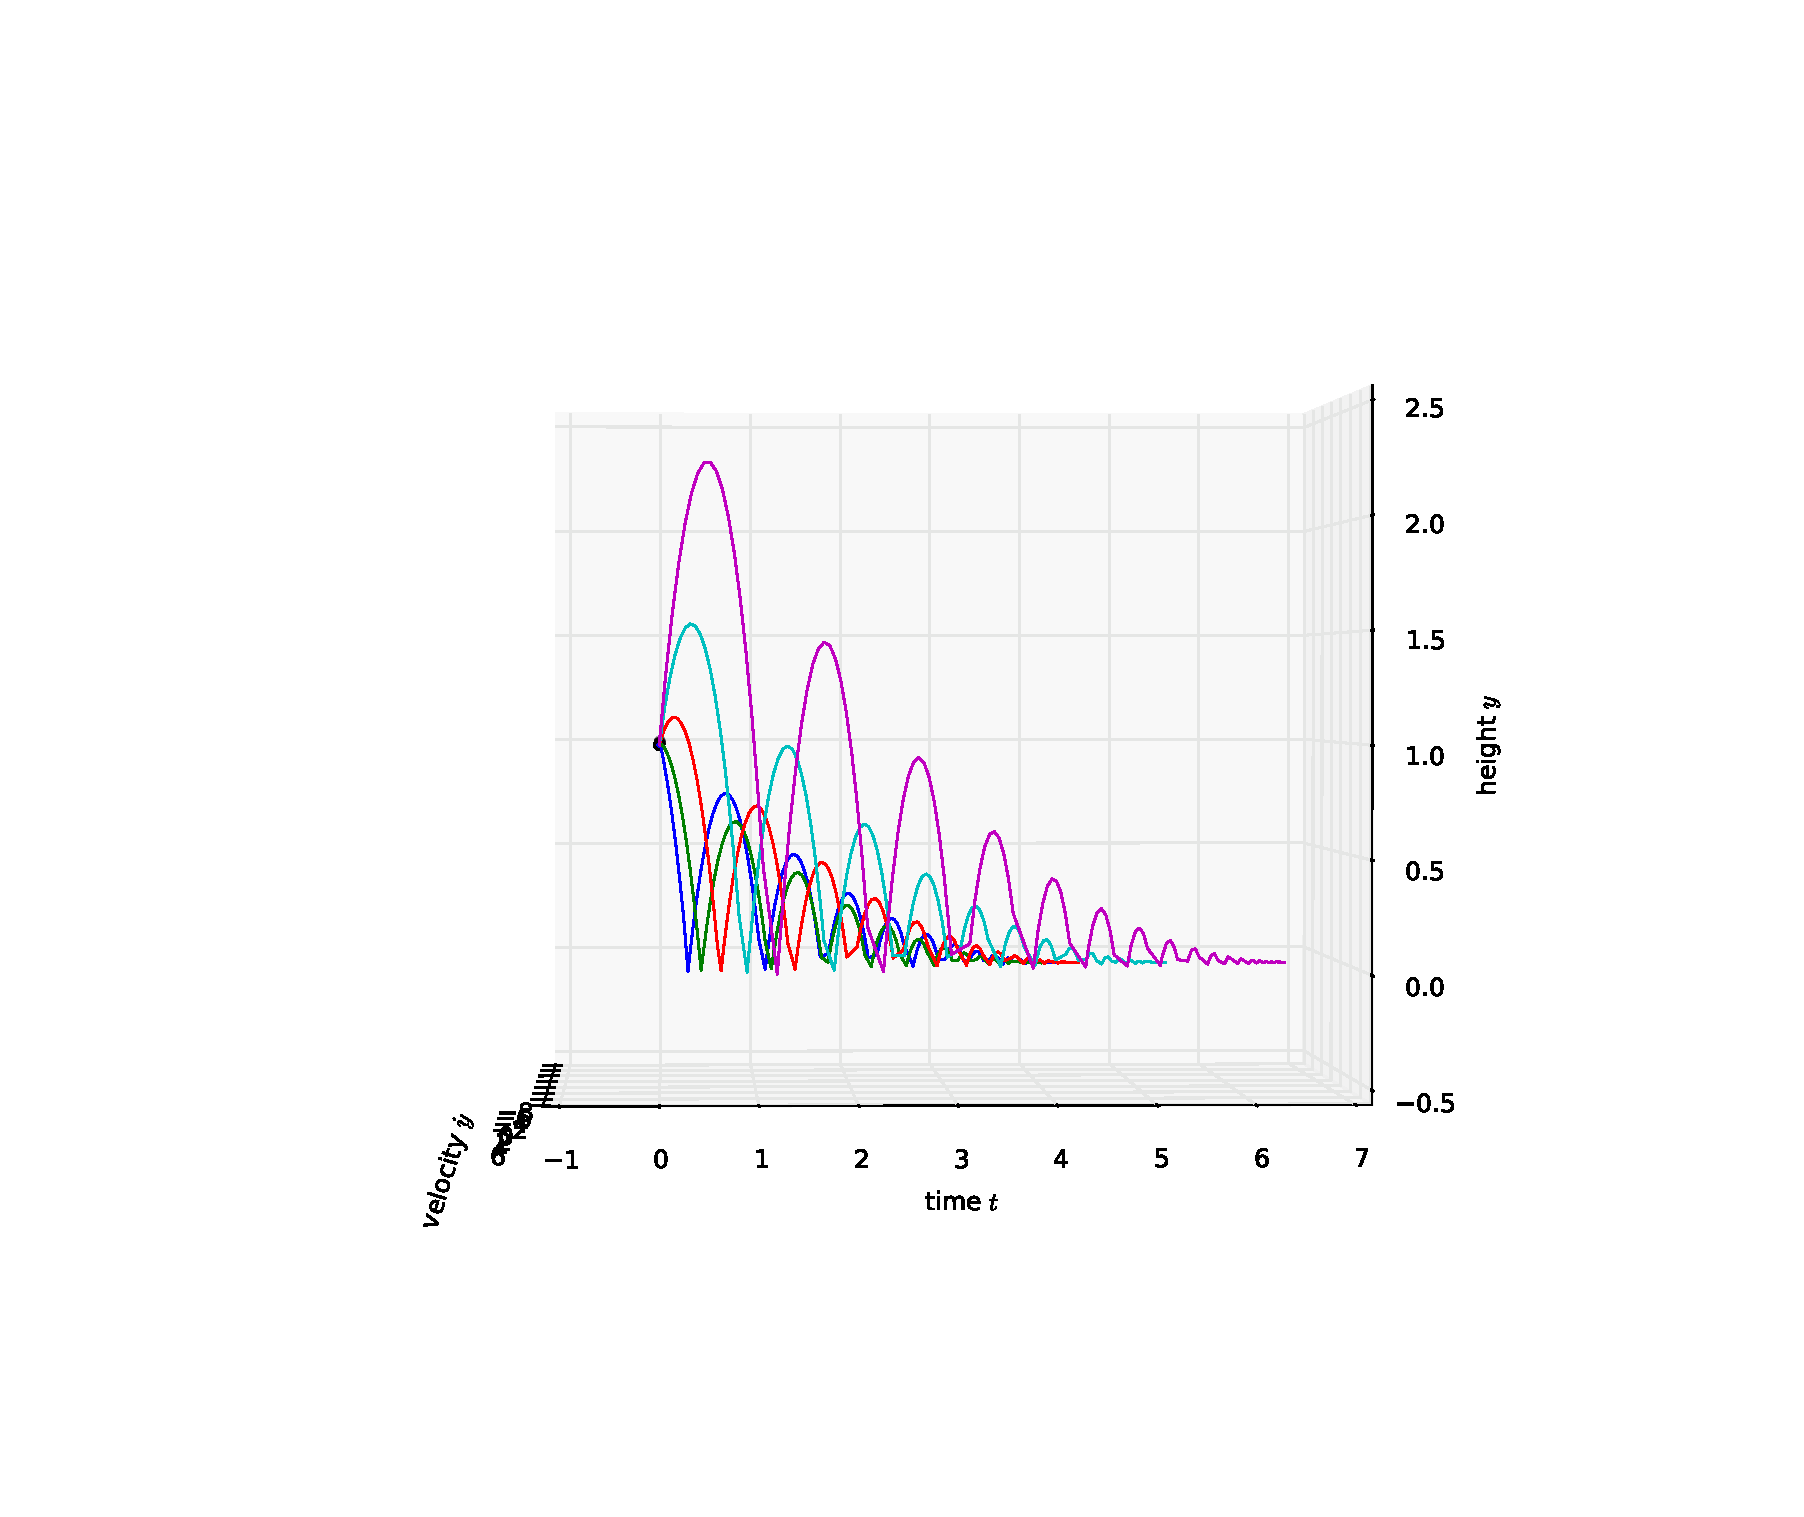
\includegraphics[width=.9\linewidth]{pic/bouncing_ball_reflattened}
\vfill\null
\end{frame}



\begin{frame}
\frametitle{A Common Class of State-Space Models}

\begin{itemize}

\vitem We begin observing a signal, or ``trajectory'',
\[
y(t) \in \reals.
\]

%\vitem We call the present moment $t=0$, and are interested in $y(t)$ over $t \geq 0$ (future).

%\vitem Many trajectories are possible, but there are ``dynamical constraints''.

\vitem Try to substitute another signal $\vecx(t) \in \reals^d$, and
functions $f : \reals^d \to \reals^d$ and $g : \reals^d \to \reals$:

\begin{enumerate}
\vitem The system
\[
\begin{cases}
	\dot \vecx = f(\vecx) \\
	\vecx(0) = \vecx_0 \qquad \text{initial condition}
\end{cases}
\]
has a unique solution over $t \geq 0$;

\vitem recover original signal over $t \geq 0$, by $y(t) = g( x(t) )$ 

%In other words, applying $g$ to the state-trajectory recovers the desired signal.

\end{enumerate}

\end{itemize}

\vfill\null
\end{frame}







\makecommand{\doequil}{
\includegraphics[width=1cm]{pic/equilibrium.jpg}}


\section{Equilibria}

\begin{frame}
\vfill
\centering

\begin{tabular}{ccccccc}
%& & \doequil & & \doequil \\
&\doequil & & & \doequil & \doequil & \\
& \doequil & & {\Large EQUILIBRIA} & \doequil & & \\
& &\doequil &\doequil & & \doequil & \\
%& &\doequil & & \\
\end{tabular}

\vfill\null
\end{frame}



\begin{frame}
\frametitle{Equilibria}

\begin{itemize}

\vitem \emph{Equilibria} are conditions such that the system ``stays put''.

\vitem Given a state-space $X$, the equilibria are 
\[
\left\{
	\vecx : \ f(\vecx) = \zerovec \implies \dot \vecx = \zerovec
\right\}
\]

\vitem Where in the wide, wide state-space will the system rest?

\end{itemize}

\end{frame}



\begin{frame}


\centering
\emph{Equilibrium for the bouncing ball?}

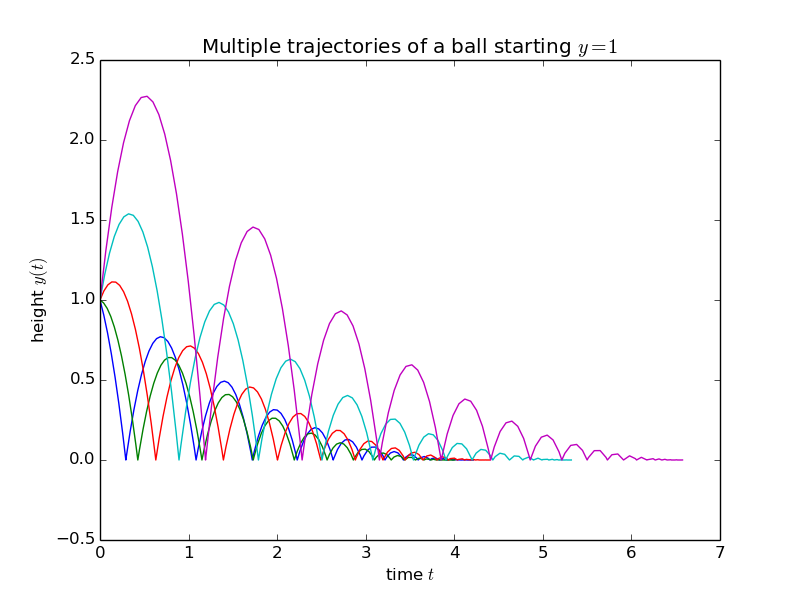
\includegraphics[width=.7\linewidth]{pic/bouncing_ball_flat}

$y(0)=1$, $\dot y(0)$ various

\end{frame}



\begin{frame}
\frametitle{Ideal Pendulum System}

\begin{columns}

\column{.45\linewidth}

Pendulum trajectories satisfy

$\ddot\theta + (g/l) \sin \theta = 0$.

Use angle and angular velocity as a state-space.

$\vectheta = (\theta, \dot \theta)^\xpose$

$f(\vectheta)
	= \begin{pmatrix}
		\dot\theta \\
		-\frac{g}{l} \sin\theta
	\end{pmatrix}$.
	
$g > 0$ (thanks, universe), so:

\[
\begin{cases}
\dot\theta = 0 \\
\sin \theta = 0
\end{cases}
\]

\column{.45\linewidth}

\begin{center}
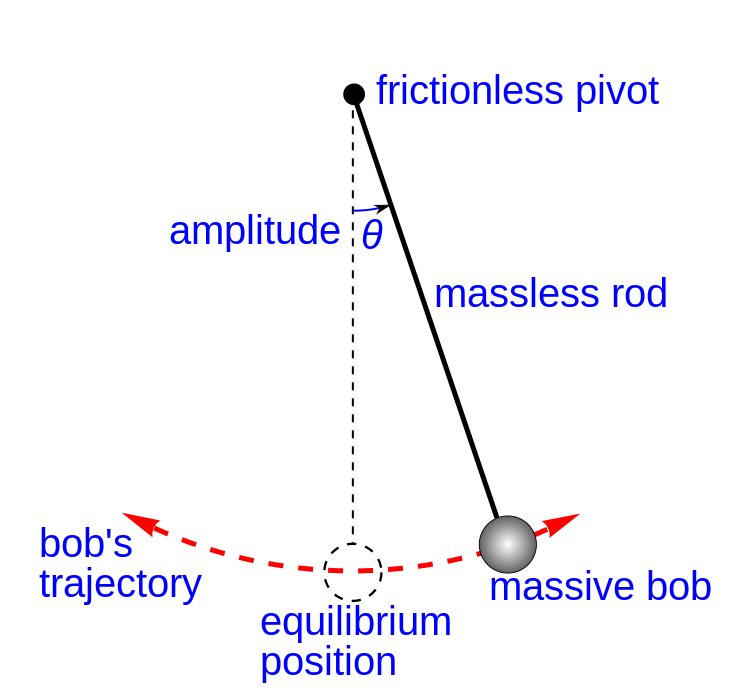
\includegraphics[width=\linewidth]{pic/Simple_gravity_pendulum.png}
\end{center}

\end{columns}

\end{frame}














\begin{frame}
\frametitle{Equilibria of the Pendulum}

Two [physically] distinct equilibria:

\begin{columns}

\column{.45\linewidth}

\begin{center}
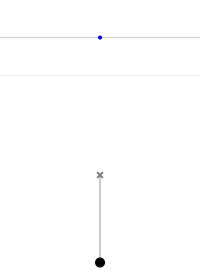
\includegraphics[width=.4\linewidth]{pic/Pendulum_0deg.png}

$\dot\theta = 0$, $\theta=0$

\end{center}


\column{.45\linewidth}

\begin{center}
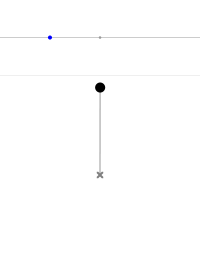
\includegraphics[width=.4\linewidth]{pic/Pendulum_180deg.png}

$\dot\theta = 0$, $\theta=\pi$
\end{center}


\end{columns}

\vfill
But we have a gut feeling that one of these equilibria is not ``stable''.

\end{frame}








\section{Stability}

\subsection{Introduction}

\begin{frame}
\frametitle{Stability}

\begin{itemize}

\vitem Stability is a property of \emph{equilibria}, \emph{not} systems!

\vitem Stability of ``systems'' is a colloquialism which arose because of the importance of \emph{linear} systems;

\vitem Linear systems tend to have unique equilibrium (at origin).

\vitem But, it doesn't make any sense to ask \emph{``Is the pendulum stable?''}

\end{itemize}

\end{frame}



\subsection{Definition}

\begin{frame}
\frametitle{Lyapunov Stability}
\vfill
\begin{block}{Informal}
``If I put it there, and then I go make a sandwich, will it be like that when I get back?''
---Kyle
\end{block}

\vfill
\begin{block}{Formal}
An equilibrium $\bar\vecx$ is said to be \textbf{stable in the sense of Lyapunov} if:
for every $\epsilon > 0$, there is $\delta >0$, so that
if $\vecnorm{\vecx(0)-\bar\vecx} < \delta$, then
$\vecnorm{\vecx(t) - \bar\vecx} < \epsilon$. 
\end{block}

\vfill\null

\end{frame}





\begin{frame}
\frametitle{Break-down}

\begin{block}{Formal}
$\bar\vecx$ is \textbf{stable in the sense of Lyapunov} if
\emph{for every $\epsilon > 0$}, there is $\delta >0$, so that
$\vecnorm{\vecx(0)-\bar\vecx} < \delta
 \implies \vecnorm{\vecx(t) - \bar\vecx} < \epsilon$. 
\end{block}

\begin{tabular}{rp{.6\linewidth}}
$\vecnorm{\vecx(0)-\bar\vecx}$
	& Initial distance from the equilibrium state \\ \\
	
$\vecnorm{\vecx(t)-\bar\vecx}$
	& Distance from the equilibrium state at time $t$ \\ \\
	
$\vecnorm{\vecx(0)-\bar\vecx} < \delta$
	& Start close; then... \\ \\

$\implies \vecnorm{\vecx(t)-\bar\vecx} \leq \epsilon$
	& Stay close (for all $t \geq 0$). \\

\end{tabular}

\vfill\null

\end{frame}





\begin{frame}
\frametitle{Other Properties of Equilibria}

\begin{block}{Attractive}
If there is $\delta > 0$ so that if $\vecnorm{\vecx(0)-\bar\vecx} < \delta$, then
$\vecnorm{\vecx(t)-\bar{\vecx}} \to 0^+$.
\end{block}

\begin{block}{\emph{Asymptotically} Stable}
Stable in the sense of Lyapunov \emph{and} attractive.

(Attractive does not imply i.s.L.)
\end{block}

\begin{block}{Exponentially Stable}
If there are $\alpha, \beta, \delta >0$, so that if
$\vecnorm{\vecx(0)-\bar{\vecx}} < \delta$, then
$\vecnorm{\vecx(t)-\bar\vecx}
	\leq \alpha \vecnorm{\vecx(0)-\bar\vecx} e^{-\beta t}$
\end{block}

\end{frame}




\begin{frame}
\frametitle{Pathology?}
\end{frame}



\subsection{Direct Method}

\begin{frame}
\frametitle{Lyapunov's Second (``Direct'') Method}

\begin{itemize}
\vitem
It can be challenging, tedious, or impossible
to prove such claims about ``all trajectories'';
even to \emph{find} them (pendulum!).

\vitem
Lyapunov's ``direct'' method can provide a short-cut.
(State-space comes to the rescue again.)

\end{itemize}

\vfill\null
\end{frame}


\begin{frame}
\frametitle{Functions of State}

\begin{itemize}
\vitem
Let $V : \reals^d \to \reals$ be a \emph{continuous}, scalar ``state'' function.

%\vitem
\[
\begin{aligned}
\doteq \dot V(t) = 
\timederiv V(\vecx(t))
	&= \frac{\partial V}{\partial \vecx} (\vecx(t)) \times \frac{d\vecx}{dt}	\\
	&= \nabla_\vecx V(\vecx(t)) \cdot \dot\vecx	\\
	&= \nabla_\vecx V(\vecx(t)) \cdot f(\vecx(t))	\\
%	&\doteq \dot V(\vecx(t)).
\end{aligned}
\]

%\begin{block}{Lyapunov}
%\begin{enumerate}
\vitem
Unlike trajectories, $V$, $\dot V$ are often obtainable;
(after all, we have some choice in $V$)
%e.g., if we can choose $V$ from a family of functions whose partial derivatives we can compute

\vitem
$\dot V$ is \emph{also} a ``state function''; given $\vecx$, doesn't depend on $t$

\vitem
Lyapunov theorems usually of the form

If $V$ and $\dot V$ satisfy some conditions,

then, trajectories of the system satisfy some other conditions.

%\end{enumerate}
%\end{block}
\end{itemize}

\end{frame}









\begin{frame}
\frametitle{Lyapunov candidates}

\begin{itemize}

%\vitem
%Let $V : \reals^d \to \reals$ be a \emph{continuous}, scalar function.

\vitem
$V$ is a Lyapunov candidate if is \emph{positive-definite}, i.e.,

\[
\begin{cases}
	V(\zerovec) = 0 &\\
	V(\vecx) > 0 & \text{for all $\vecx \neq \zerovec$}.
\end{cases}
\]

\vitem
May be positive definite \emph{locally}; i.e., in a ``neighborhood''
(open set, containing $\zerovec$)

\vitem
(Assuming \emph{without loss of generality} that $\bar{\vecx} = \zerovec$.)

\end{itemize}
\vfill\null
\end{frame}




\begin{frame}
\frametitle{Definiteness}

5. Define and demonstrate [positive/negative] [semi-] definiteness.

(6. Define and demonstrate sub-level sets?)

\end{frame}












\begin{frame}



\end{frame}





\begin{frame}
\frametitle{Pendulum Example}

(put the pendulum energy picture)

\[
E = mgh + \onehalf m v^2.
\]

$h = l(1-\cos\theta)$

$v = (l\dot\theta)^2$

\[
E
%ml \, g(1-\cos\theta) + \onehalf ml^2 \, \dot\theta^2
	= ml \left( g \, (1-\cos\theta) + \onehalf l \, \dot\theta^2 \right)
\]

\[
E' = g \, (1-\cos\theta) + \onehalf l \, \dot\theta
\]

(plot the surface, show positive definite!)

\end{frame}



\begin{frame}
\frametitle{Pendulum Example}
\[
\frac{\partial}{\partial\theta} E' = g \sin \theta
\]

\[
\frac{\partial}{\partial\dot\theta} E' = l \dot\theta
\]

\[
\dot E' =
	\frac{\partial}{\partial\theta} E' 
		\times f_{\theta}(\vectheta)
	+ \frac{\partial}{\partial\dot\theta} E'
		\times f_{\dot\theta}(\vectheta)
\]


\[
\dot E' =
	\left( g \sin\theta \times \dot\theta \right)
	+ \left( l \dot\theta \times (-g/l) \sin \theta \right) = 0
\]

(This is something we expected, being familiar with physics and conservation of total energy.)

Proof that the bottom equilibrium is stable i.s.L.; but \emph{not} attractive

\end{frame}










\begin{frame}
\frametitle{Review of Last Time: Second-order State-space Model}

\begin{center}
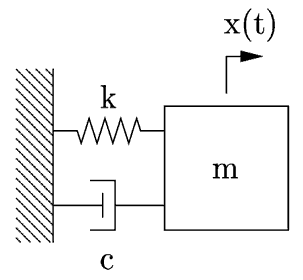
\includegraphics[width=.3\linewidth]{pic/spring-mass-damper.png}
\end{center}

\begin{block}{Second-order, Linear Dynamical System}
$u(t)$ describes the position of a mass over time.

Known to obey the law:
$m \ddot u = -k u - c \dot u
	\implies\qquad
	\ddot u = -(k/m) u - (c/m) \dot u$,
	
where $\dot u = \timederiv u(t)$ (velocity), $\ddot u = \frac{d^2}{dt^2} u(t)$ (acceleration).
\end{block}

\end{frame}






\begin{frame}
\begin{block}{State-space Model}
Write
$\vecu(t) = \left( u(t), \dot u(t) \right)^\xpose$;
also written, 
$\vecu = \begin{pmatrix} u \\ \dot u \end{pmatrix}$.

(Element-wise derivative)

$\dot\vecu
	\doteq \timederiv \vecu(t)
	= ( \timederiv u(t), \timederiv \dot u(t) )^\xpose
	= \begin{pmatrix}
		\dot u \\
		\ddot u
	\end{pmatrix}$.

\end{block}

\begin{block}{SMD Model}
$\dot \vecu
	= \begin{pmatrix} \dot u \\ \ddot u \end{pmatrix}
	= \begin{pmatrix}
		\dot u \\
		-(k/m) u - (c/m) \dot u
		\end{pmatrix}$
		
$\dot \vecu
	= \begin{pmatrix} \dot u \\ \ddot u \end{pmatrix}
	= \begin{pmatrix}
		\dot u \\
		-(k/m) u - (c/m) \dot u
		\end{pmatrix}
	= \begin{pmatrix} 0 & 1 \\ -\frac{k}{m} & -\frac{c}{m} \end{pmatrix}
	\vecu$.
	
\end{block}

\end{frame}


\begin{frame}
\frametitle{SMD Equilibrium}

\begin{itemize}
\vitem In our example:
\[
f(\vecx) = \zerovec \implies
\begin{cases}
	\dot u = 0	\\
	\ddot u = -(k/m) u - (c/m) \dot u = 0
\end{cases}
\]

\vitem If $k > 0$, equilibrium of $u = 0$ and $\dot u = 0$ is \emph{unique}.

\vitem If $k = 0$, all $u$ are equilibria when $\dot u = 0$.
\end{itemize}
\end{frame}


\begin{frame}

\begin{itemize}

\vitem
$\matA := \begin{pmatrix} 0 & 1 \\ -\frac{k}{m} & -\frac{c}{m} \end{pmatrix}$

\vitem
Then $\dot\vecu$ is given by $f(\vecu) = \matA \vecu$

\vitem $\matC := \begin{pmatrix} 1 & 0 \end{pmatrix}$

\vitem
Then $u(t)$ is given by
$g(\vecu) = \matC \vecu$.

\end{itemize}
\vfill\null

\end{frame}


\begin{frame}
\frametitle{Solution}

\begin{itemize}

\vitem Admits a unique state-space trajectory determined by initial conditions $\vecu(0) = \vecu_0$
\[
  \vecu(t) = \vecu_0 e^{t \matA }
  \qquad t \geq 0.
\]

\vitem Particle trajectory is given by $u(t) = \matC \vecu(t)$ for $t \geq 0$.

\end{itemize}
\vfill\null

\end{frame}




\begin{frame}
Put ``state-space'' locus plots of equilibria in the two cases.
\end{frame}





\begin{frame}
\frametitle{Stability for LTI Systems (Continuous)}


Can I find $P$ and $Q$ which are p.d., n.[s.]d simultaneously?

$\dot x = Ax$

The notation $P > 0$ means that matrix P is positive definite.
Given any $Q > 0$, there exists a unique $P > 0$ satisfying 
$A^\xpose P + P A + Q = 0$ if and only if the origin is the globally asymptotically stable equilibrium of the linear system $\dot x = A x$.

If and only if $\lambda \in eig(A) => Re(\lambda) < 0$

The quadratic function $V(z) = z^\xpose P z$ is a Lyapunov function that can verify stability.

\emph{Otherwise, unstable!}

\end{frame}






\begin{frame}
\frametitle{Discussion}

\begin{itemize}
\vitem
There is an instability theory

\vitem
Similar theories for discrete systems (e.g., computer programs);
hybrid systems (bouncing ball)

\vitem A lot of this material cribbed from

\url{http://stanford.edu/class/ee363/lectures/lyap.pdf}
\end{itemize}



\end{frame}









\begin{frame}
BACKUP
\end{frame}




\makecommand{\matJ}{{\bf J}}

\begin{frame}
\frametitle{Lyapunov's Indirect Method (Linearization)}

Given $\dot \vecx = f(\vecx)$ and equilibrium $\vecx_e$,
form system

$\tilde\vecx = \vecx - \vecx_e$

$\dot{\tilde\vecx}
	= \left.
		\frac{\partial f }{\partial\vecx} \right|_{\vecx=\vecx_e}
		\, \tilde\vecx$.



$\dot V \prec 0$ means stable;

$\dot V \preceq 0$ is undecided;

$\dot \succ 0$, but $\dot V \neq 0$ means unstable;

(Could use this one against the pendulum inverted equilibrium?)

\end{frame}







\begin{frame}
\frametitle{Rosenbrock-transformed Spring-Mass-Damper}

\begin{equation}
V = b \left( y - x^{2}\right)
	\left(
		-\onehalf a + \frac{b}{2c} \left(k + m\right) \left(- x^{2}{\left (t \right )} + y{\left (t \right )}\right) + 0.5 x{\left (t \right )}\right)
		+ \left(a - x{\left (t \right )}\right) \left(- 0.5 b \left(- x^{2}{\left (t \right )} + y{\left (t \right )}\right) + \frac{0.5}{c k} \left(a - x{\left (t \right )}\right) \left(c^{2} + k m + m^{2}\right)\right)
\end{equation}

\begin{equation}
\dot V = -b^2 \left( y - x^2 \right) - \left( a - x \right)^2
\end{equation}

\end{frame}













\end{document}